%----------------------------------------------------------------------------
\chapter{Implementáció}
\label{chp:implementation}
%----------------------------------------------------------------------------
\begin{itemize}
  \item a két alfejezet rövid tartalma jön ide, + a repo elérhetősége
\end{itemize}

%----------------------------------------------------------------------------
\section{A fájlterítő alkalmazás}
%----------------------------------------------------------------------------

%
\subsection{Felhasználói felület}
%
\begin{itemize}
  \item parancssorból indítható jar fájl, terítés utolsó fázisában avatkozhat be a felhasználó (a torrent-alapú fájlátvitel közben)
\end{itemize}

%
\subsection{Az alkalmazás osztályai}
%



\begin{itemize}
  \item A funkcionalitás szempontjából jelentősebb osztályok bemutatása, komplexebb kódrészletek magyarázata
\end{itemize}

%----------------------------------------------------------------------------
\section{Terítés szereplőinek konfigurációja}
%----------------------------------------------------------------------------

\begin{itemize}
  \item Ezekben a fejezetekben mutatom be, hogy a program működéséhez az egyes gépeken milyen szkripteket kell futtatni, milyen programokat kell telepteni
\end{itemize}


%
\subsection{Nem kiemelt laborgépek}
%

\begin{itemize}
  \item ``sima'' laborgépek konfigurációja, ez főleg a torrentkliens teleptéséből, és annak konfigurálásából áll (hogy távolról is lekérdezhető legyen annak aktuális állapota)
\end{itemize}

%
\subsection{Kiemelt laborgép (seed)}
%

\begin{itemize}
  \item Az előbbiekhez még a torrent tracker telepítése és a vezérlést végző bash szkriptek bemutatása jön hozzá
\end{itemize}


%----------------------------------------------------------------------------
\section{Egy konkrét terítés végigkövetése}
%----------------------------------------------------------------------------

A tesztelést a program fejlesztésére használt gépen végeztem el, a terítésben résztvevő gépek Vagrant-tal létrehozott, VirtualBox\cite{virtualbox} által futtatott virtuális gépek, amelyeken az operációs rendszer 32-bites 12.04 verziójú Ubuntu\cite{ubuntu}. A virtuális gépekre csak a legszükségesebb szoftverek lettek telepítve, egymással és a gazdagéppel egy közös privát hálózaton voltak. A program futtatásához megadott labormodell fontosabb paraméterei:

\begin{itemize}
  \item Két különböző virtuális gép van benne: egy mi általunk és egy Vagrant által készített
  \item 6 számítógép, amik közül az egyik dedikált seed (labpc101-105, seed nevűek)
  \item Olyan célállapot, amivel minden lehetséges hiba meg fog jelenni a futás során
\end{itemize}

Mielőtt végigkövetnénk a futtatást érdemes végiggondolni, hogy mi lenne az elvárt eredmény, milyen fontosabb lépéseket és milyen sorrendben fog a program végrehajtani:

\begin{enumerate}
  \item Figyelmeztetés, hogy 105 és 104-re semelyik, 103 és 102-re pedig egyik virtuális gép nem fog terülni bizonyos problémák miatt
  \item Vagrant-os VM inicializálása, majd becsomagolása egy .zip archívumba
  \item Mindkét VM felmásolása a seed gépre, mindkettőhöz torrent fájl létrehozása
  \item Torrentkliens futtatása a seed gépen
  \item Torrent fájlok átmásolása a labpc101-103 gépekre
  \item Torrentkliens futtatása a labpc101-103 gépeken
  \item A letöltések sikeres befejezése után a modell frissítése
\end{enumerate}

A program indítása után rögtön a várt figyelmeztetések jelennek meg a konzolablakban:\\\\
\code{2015-12-08 00:21:48 WARNING hu.bme.mit.vmdistribution.app.EMFModelUtil isCompatible WARNING:\_Computer:labpc104 is not compatible with Virtual Machine:vagrantvm\_test, Not enough RAM!}\\
\code{2015-12-08 00:21:48 WARNING hu.bme.mit.vmdistribution.app.EMFModelUtil isCompatible WARNING:\_Computer:labpc104 is not compatible with Virtual Machine:customvm\_test, Not enough RAM!}\\
\code{2015-12-08 00:21:48 WARNING hu.bme.mit.vmdistribution.app.EMFModelUtil isCompatible WARNING:\_Computer:labpc103 is not compatible with Virtual Machine:vagrantvm\_test, Architecture mismatch!}\\
\code{2015-12-08 00:21:48 WARNING hu.bme.mit.vmdistribution.app.EMFModelUtil hasEnoughSpace WARNING:\_Computer:labpc105 does not have enough free space for the new VMs! Available: 2000.0 MB, Required: 15500.0 MB}\\\\
Majd meghívódik a Vagrant és létrehozza, valamint beállítja a hozzá tartozó VM-et. \Aref{fig:vboxcap}-es~ábrán látható, hogy a VirtualBox VM-eket tartalmazó mappájába már bele is került az új virtuális gép és meg is jelenik annak a felületén.

\begin{figure}[ht]
\centering
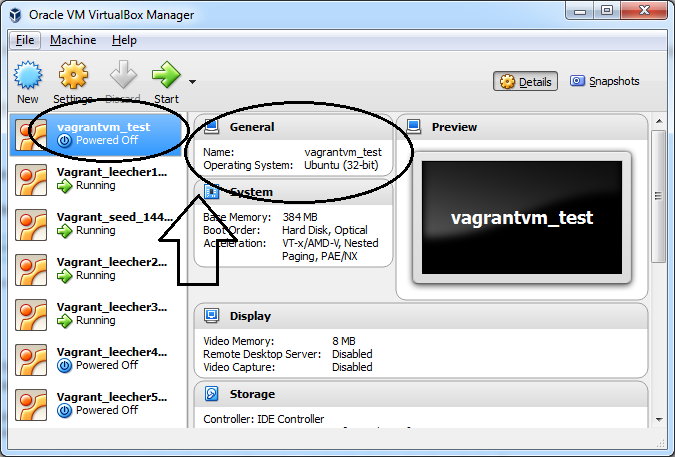
\includegraphics[width=100mm, keepaspectratio]{figures/test_vbox.png}
\caption{Vagrant által létrehozott virtuális gépek a VirtualBox-ban}
\label{fig:vboxcap}
\end{figure}
A kész virtuális gépből a program létrehoz egy tömörített .zip állományt\ldots\\\\
\code{2015-12-08 00:37:03 INFO hu.bme.mit.vmdistribution.app.vmutil.Archiver createZipArchive Creating Archive: E:\textbackslash{}vagrantvm\_test.zip}\\\\
\ldots majd a két VM felkerül a seed-re, ahogy \aref{fig:seed_files}-es~ábrán ez látszik is:  a seed-del SSH kapcsolat létesítése után kilistázzuk azoknak a mappáknak a tartalmát ahová a VM-eket tartalmazó zip fájlok, illetve az azok alapján készített torrent fájlok kerültek.

\begin{figure}[ht]
\centering
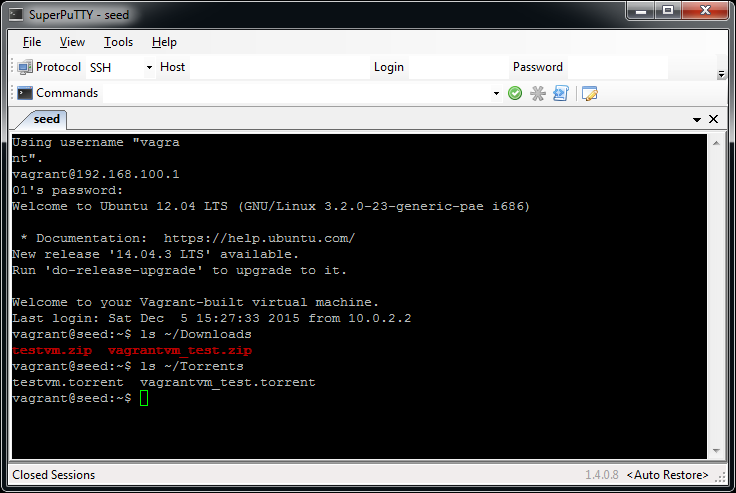
\includegraphics[width=120mm, keepaspectratio]{figures/test_seed_files.png}
\caption{Terítendő VM-ek és a torrent fájlok a seed-en}
\label{fig:seed_files}
\end{figure}

Ezután az alkalmazás a torrent fájlokat átmásolja a megfelelő célgépekre, és elindítja rajtuk a torrentklienst. A seed-en futó torrentklienst megnyitva ellenőrizhetjük, hogy elkezdődött-e az adatátvitel (\ref{fig:seed_torrent}. ábra). A feltöltési limit kézzel alacsonyra lett állítva, hogy a folyamatok megfigyelhetőek legyenek.

\begin{figure}[ht]
\centering
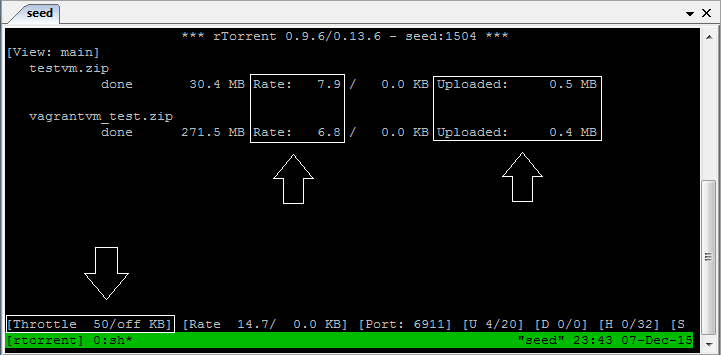
\includegraphics[width=120mm, keepaspectratio]{figures/test_seed_torrent.png}
\caption{Rtorrent: Futó feltöltések}
\label{fig:seed_torrent}
\end{figure}

A két futó fájlátvitel részleteit megnézve ellenőrizhetjük, hogy a megfelelő gépek töltenek-e le. Például a mi általunk készített VM-et tartalmazó testvm.zip-et a labpc101 és 103-nak kellene töltenie, lásd \ref{fig:seed_peers}-es~ábra (a két gép IP címe .111 ill. .113-ra végződik).

\begin{figure}[ht]
\centering
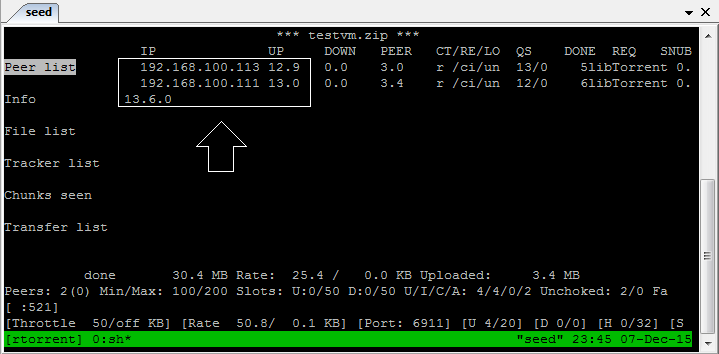
\includegraphics[width=120mm, keepaspectratio]{figures/test_seed_peers.png}
\caption{Rtorrent: Torrent részletei}
\label{fig:seed_peers}
\end{figure}

Egy pár percen belül véget is ér a terítés:\\\\
\code{2015-12-08 00:46:40 INFO hu.bme.mit.vmdistribution.app.distrstatus.DistributionStatusUpdater run [All transfers are finished, distribution is complete, press ENTER to continue.]}\\
\code{2015-12-08 00:46:57 INFO hu.bme.mit.vmdistribution.app.UseModel main [Saving changes to model instance.]}\\
\code{2015-12-08 00:46:57 INFO hu.bme.mit.vmdistribution.app.UseModel main [Done.]}\\\\

A modellünket tartalmazó fájlt közelebbről megnézve ellenőrizhetjük, hogy az tényleg frissült-e, a labpc101-et reprezentáló Computer objektum például most már így néz ki:\\\\
\code{<computers virtualmachines="//@virtualmachines.1 //@virtualmachines.0" name="labpc101" maxSpaceForVMs="40000.0" installedRAM="8000.0" architecture="x64">}\\\\
A Computer-en levő virtuális gépeket a virtualmachines lista tárolja, aminek a két eleme a terített virtuális gépek objektumaira mutat.\\

Befejeztük az alkalmazás tesztelését, az elvárt eredményre jutottunk.
